\chapter{Вычислительные эксперименты}
\section{Программа для ЭВМ}
В качестве языка программирования для рассчётов и
визуализации был выбран Python с использованием библиотек numpy
(вычисления) и matplotlib (визуализация).
\section{Явная схема (explicit)}



Явная схема использует аппроксимацию по пространству и времени на текущем слое. Дифференциальное уравнение заменяется на:
$$
	\frac{u_i^{j+1} - u_i^j}{\Delta t} + v \frac{u_{i+1}^j - u_{i-1}^j}{2\Delta x} = f_{i}^{j}.
$$

Рекуррентная формула для вычисления значений:
$$
 u_i^{j+1} = u_i^j - \frac{v \Delta t}{2 \Delta x} \left( u_{i+1}^j - u_{i-1}^j \right),
$$

Для устойчивости явной схемы необходимо выполнение условия Куранта\cite{Turchak2003}:
\begin{equation}
	\boxed{\frac{v \Delta t}{2\Delta x} \leq \frac{1}{2}}.
	\label{eq:ust1}
\end{equation}
Точность метода O($\tau + h$), где $\tau$ - шаг по времени, $h$ - шаг по пространству.
\begin{figure}[h]  % Окружение для картинки
	\centering
	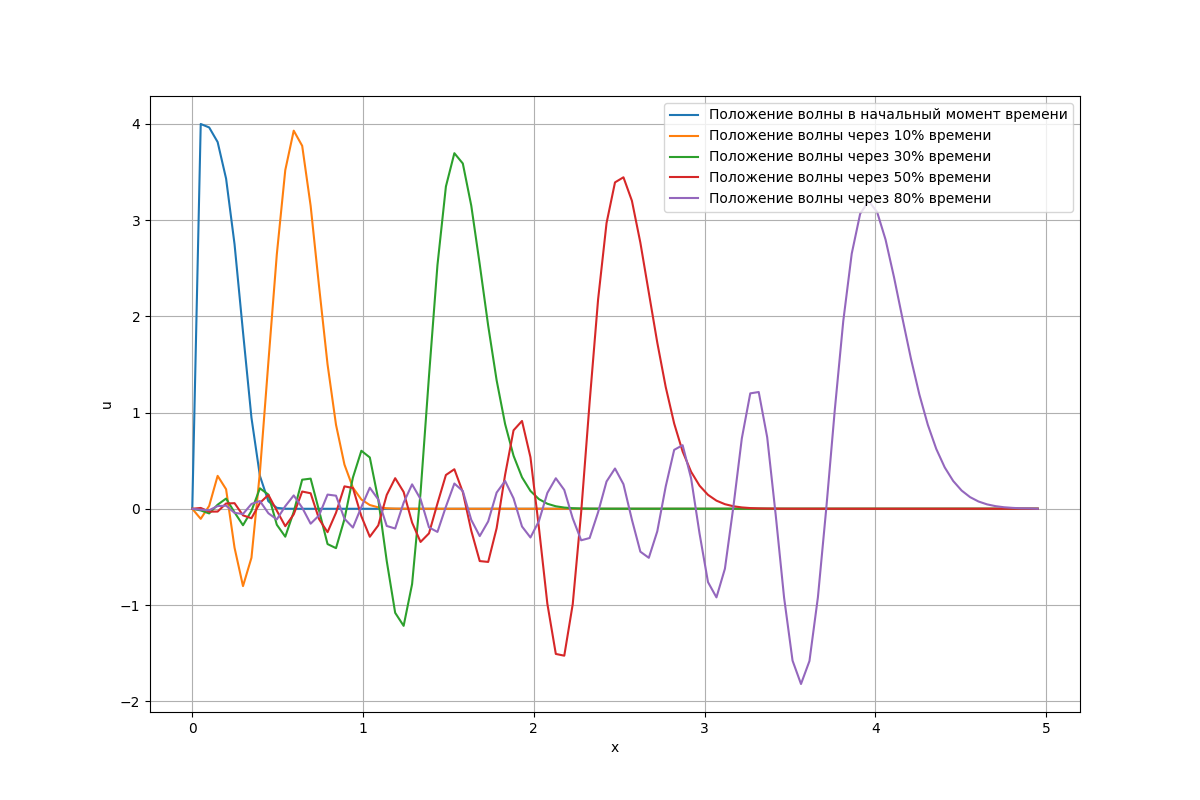
\includegraphics[height=0.7\textwidth]{imgs/explicit.png}  % Вставка изображения
	\caption{Результат решения явной схемы.$\Delta x = 0.05, \Delta t = 0.001$.}  % Подпись к изображению
	\label{fig:explicit}  % Метка для ссылки
\end{figure}
\newline
\lstinputlisting[language=Python,
captionpos=t,
]{./listings/explicit.py} 


Из представленного графика решений (рис. \ref{fig:explicit}) видно, присутствующий нисходящий тренд максимальных значений. При этом, с увеличением расстояния, пройденного волной, возникают осцилляции, с левой стороны, которые создают отрицательные значения, не имеющие физического смысла  и являющиеся одним из недостатков данной схемы решения.

Осцилляции возникают из-за дисперсионных ошибок, вызванных тем, что схема не подавляет высокочастотные компоненты и не учитывает направление переноса. Это фундаментальное ограничение центральных схем подобного рода.
\newpage
Уменьшим шаг по пространству в 1.5 раза. При таком занчении шага условие Куранта выполняется: $\frac{0.001 \cdot 1.5}{0.1} = 0.015< 0.5$.

\begin{figure}[h]  % Окружение для картинки
	\centering
	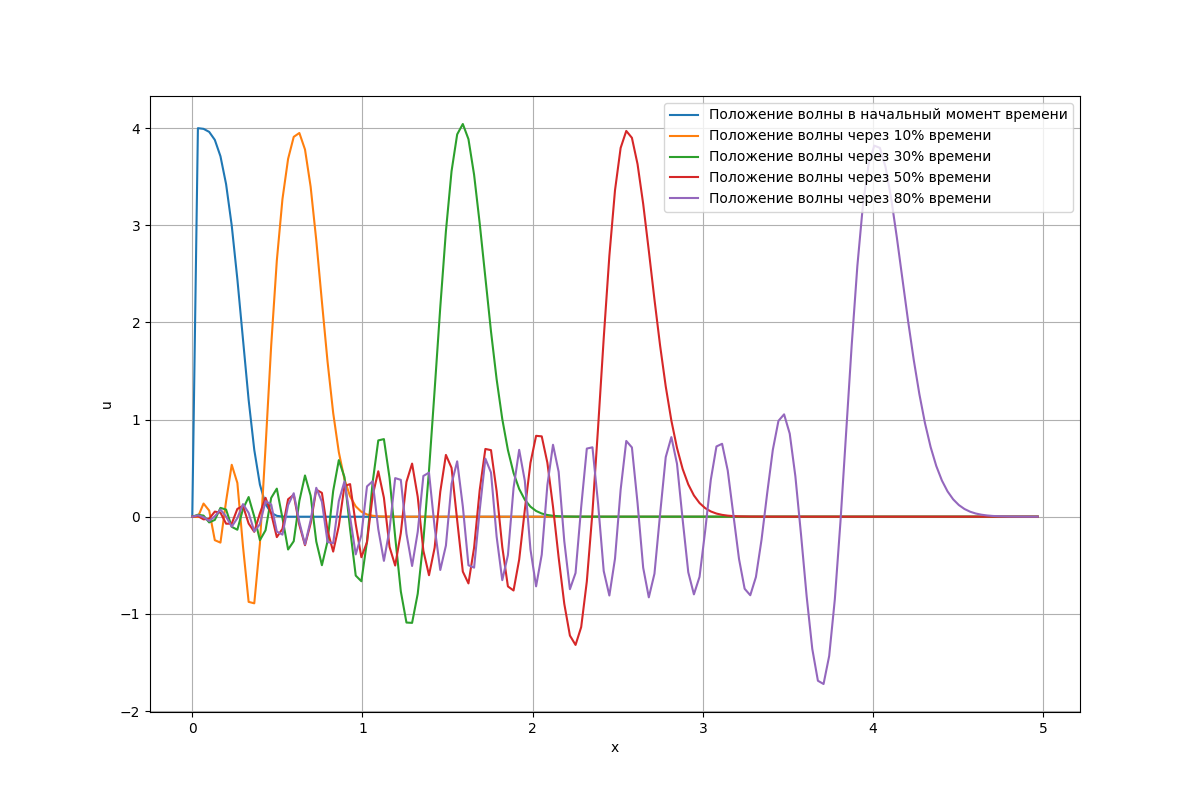
\includegraphics[height=0.7\textwidth]{imgs/explicit_1.5x.png}  % Вставка изображения
	\caption{Результат решения явной схемы. $\Delta x = 0.05 / 1.5, \Delta t = 0.001$.}  % Подпись к изображению
	\label{fig:explicit_1.5x}  % Метка для ссылки
\end{figure}
Видно (рис \ref{fig:explicit_1.5x}), что осцилляции уменьшились и пик волны уменьшается медленнее.
\newpage
Уменьшим шаг по времени в два раза. Условие Куранта сохраняется: $\frac{0.0005}{0.01} = 0.005 < 0.5$
\begin{figure}[h]  % Окружение для картинки
	\centering
	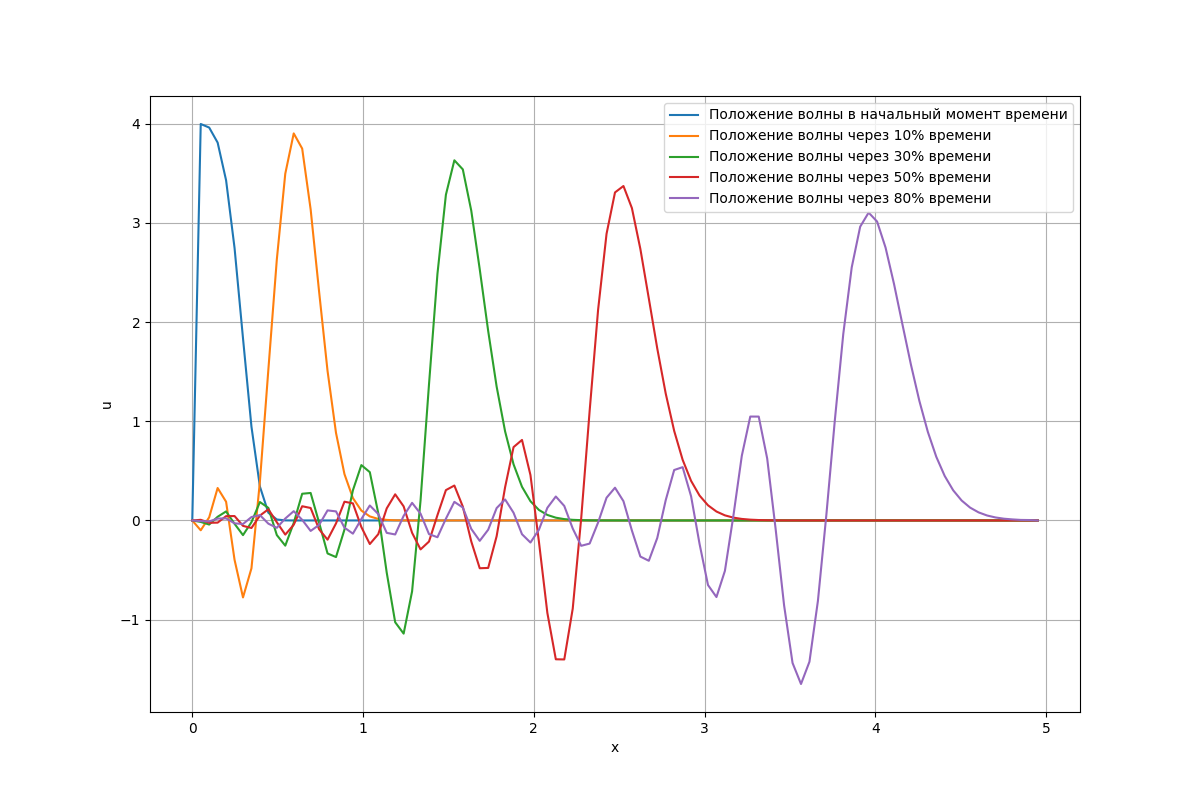
\includegraphics[height=0.7\textwidth]{imgs/explicit_2t.png}  % Вставка изображения
	\caption{Результат решения явной схемы. $\Delta x = 0.05 , \Delta t = 0.0005$.}  % Подпись к изображению
	\label{fig:explicit_2t}  % Метка для ссылки
\end{figure}

Осцилляции также уменьшились (рис. \ref{fig:explicit_2t}), но поведение пика волны не изменилось, отностельно изначальных условий
\newpage
\section{Неявная схема (implicit)}

В неявной схеме производные аппроксимируются на следующем временном слое, что обеспечивает безусловную устойчивость:
$$
	\frac{u_i^{j+1} - u_i^j}{\Delta t} + v \frac{u_{i +1}^j - u_{i-1}^j}{\Delta x^2} =  f_{i}^{j}.
$$

Результирующее уравнение можно переписать в виде линейной системы для каждого временного слоя:
$$
	- k u_{i-1}^{j+1} + u_i^{j+1} + k u_{i+1}^{j+1} = u_i^j+ \Delta t \cdot  f_{i}^{j},
$$
где $ k = \frac{v \Delta t}{ \Delta x}.$

Система уравнений имеет трёхдиагональную структуру и может быть решена методом прогонки (TDMA).
Точность метода O($\tau + h^2$), где $\tau$ - шаг по времени, $h$ - шаг по пространству.
\newline
\begin{figure}[h]  % Окружение для картинки
	\centering
	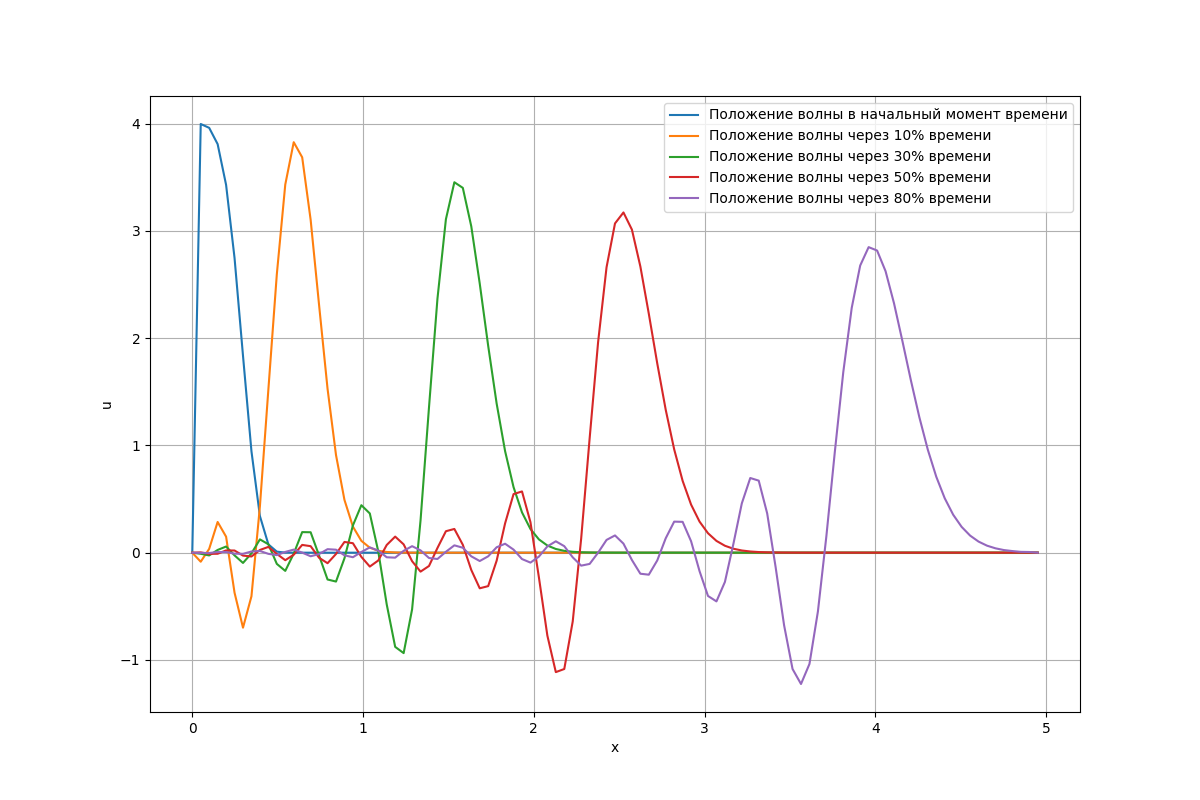
\includegraphics[height=0.7\textwidth]{imgs/implicit.png}  % Вставка изображения
	\caption{Результат решения неявной схемы. $\Delta x = 0.05 , \Delta t = 0.001$}  % Подпись к изображению
	\label{fig:implicit}  % Метка для ссылки
\end{figure}
\lstinputlisting[language=Python,
captionpos=t,
]{./listings/implicit.py} 
Рассмотрим графики решений системы (рис. \ref{fig:implicit}). В данной схеме также виден нисходящий тренд максимумов волн. И также присутствую осцилляции, хотя и меньшие по амплитуде.

\newpage
Уменьшим шаг по пространству в 1.5 раза. 

\begin{figure}[h]  % Окружение для картинки
	\centering
	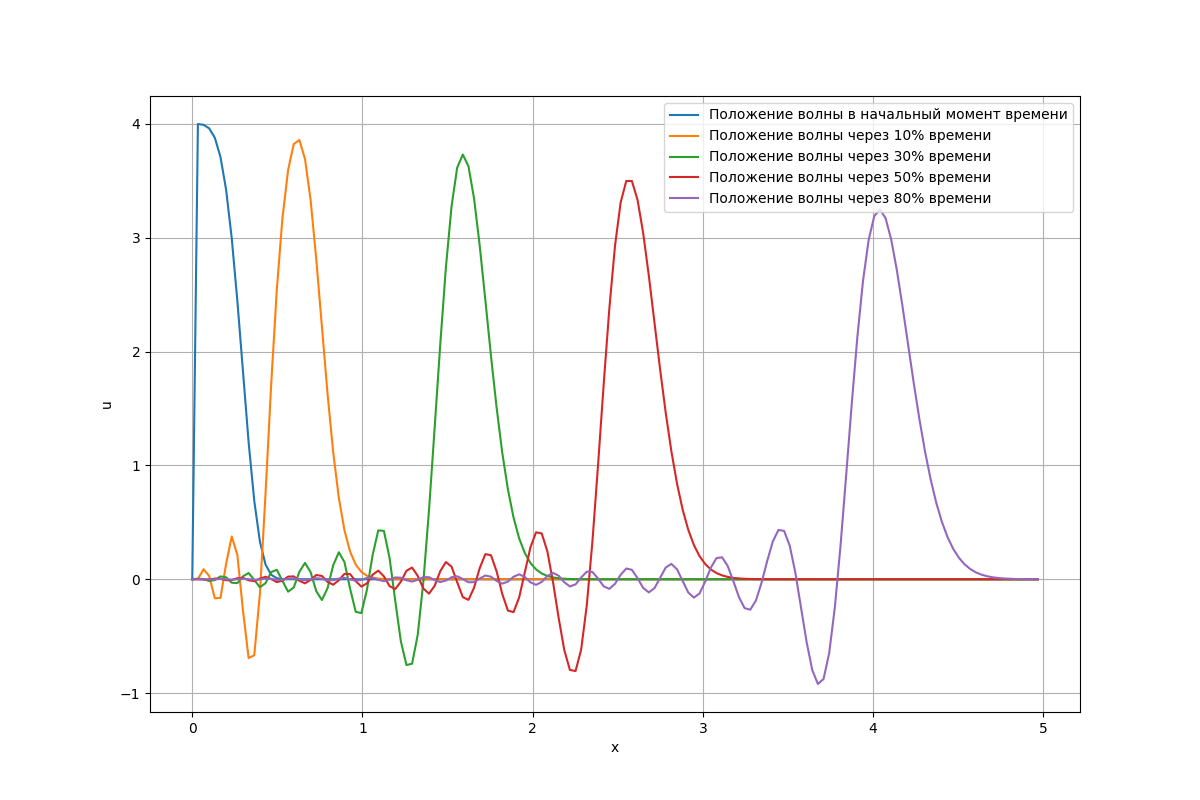
\includegraphics[height=0.7\textwidth]{imgs/implicit_1.5x.png}  % Вставка изображения
	\caption{Результат решения неявной схемы. $\Delta x = 0.05 / 1.5, \Delta t = 0.001$.}  % Подпись к изображению
	\label{fig:implicit_1.5x}  % Метка для ссылки
\end{figure}
Видно (рис \ref{fig:implicit_1.5x}), что осцилляции уменьшились и пик волны уменьшается медленнее.
\newpage
Уменьшим шаг по времени в два раза. 
\begin{figure}[h]  % Окружение для картинки
	\centering
	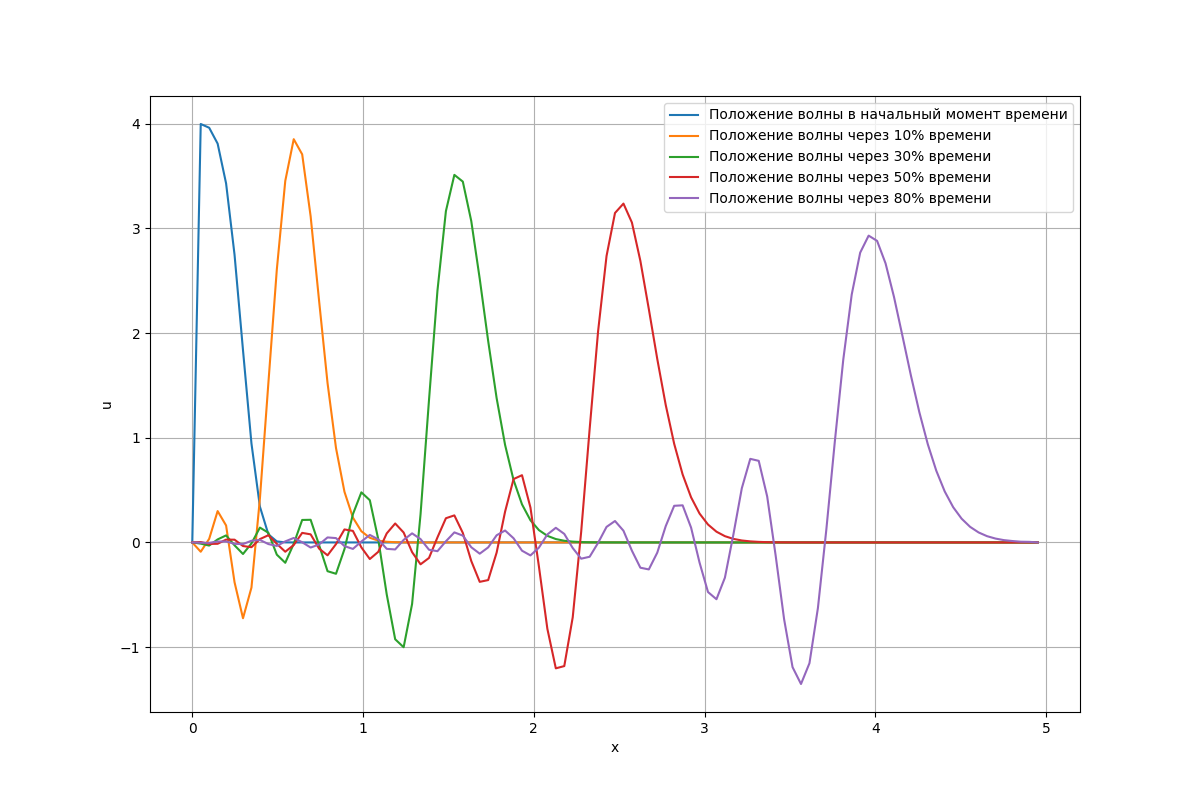
\includegraphics[height=0.7\textwidth]{imgs/implicit_2t.png}  % Вставка изображения
	\caption{Результат решения неявной схемы. $\Delta x = 0.05 , \Delta t = 0.0005$.}  % Подпись к изображению
	\label{fig:implicit_2t}  % Метка для ссылки
\end{figure}

Осцилляции также уменьшились (рис. \ref{fig:implicit_2t}), но поведение пика волны не изменилось, отностельно изначальных условий
\newpage

\section{Схема «вверх по потоку» (upwind)}

Схема «вверх по потоку» использует одностороннюю аппроксимацию производной по пространству:
$$
	\frac{u_i^{j+1} - u_i^j}{\Delta t} + v \frac{u_i^j - u_{i-1}^j}{\Delta x} = f_{i}^j.
$$

Выражая $u_i^{j+1}$:
$$
	u_i^{j+1} = u_i^j + \frac{v \Delta t}{\Delta x} \left( u_{i-1}^j - u_i^j \right).
$$

Схема стабильна при выполнении условия CFL (Курант-Фридриха-Леви)\cite{Patankar1984}:
\begin{equation}
	\boxed{\frac{v \Delta t}{\Delta x} \leq 1}.
	\label{eq:ust2}
\end{equation}
Точность метода O($\tau + h$), где $\tau$ - шаг по времени, $h$ - шаг по пространству.
\begin{figure}[h]  % Окружение для картинки
	\centering
	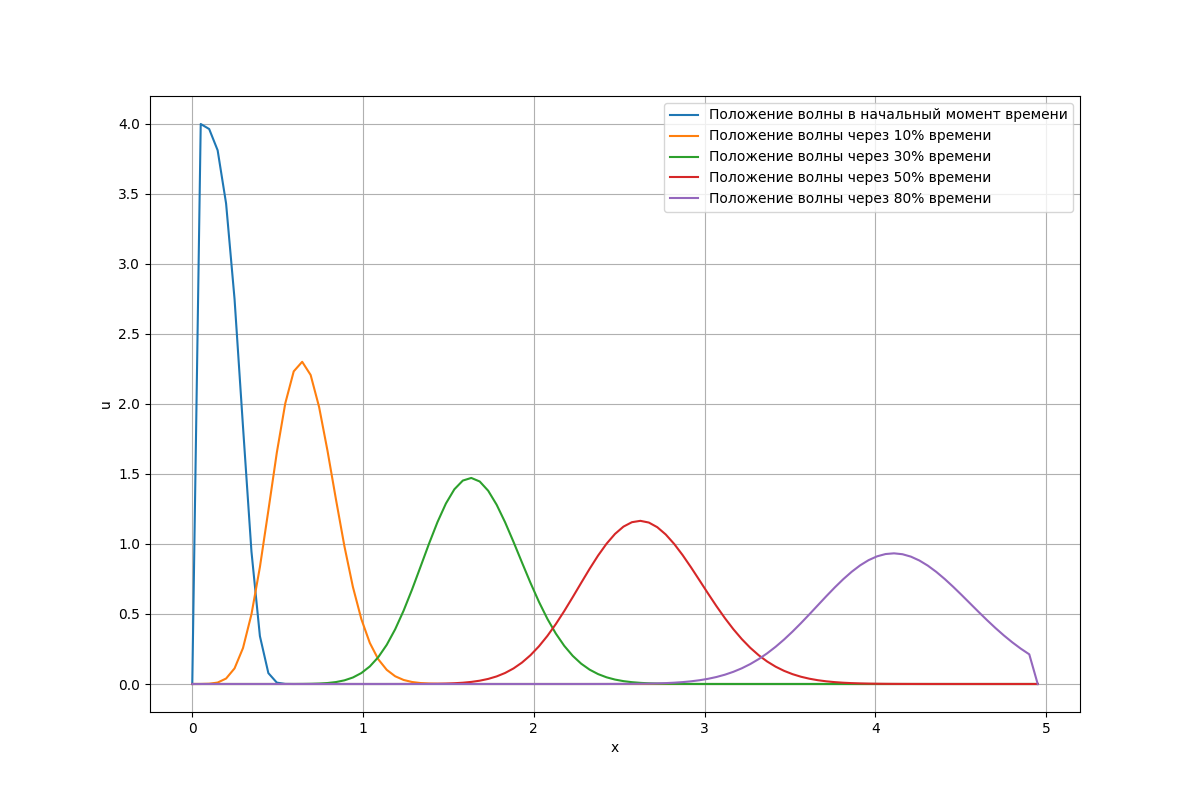
\includegraphics[height=0.7\textwidth]{imgs/upwind.png}  % Вставка изображения
	\caption{Результат решения  схемы "вверх по потоку". $\Delta x = 0.05 , \Delta t = 0.001$}  % Подпись к изображению
	\label{fig:upwind}  % Метка для ссылки
\end{figure}
\newline
\lstinputlisting[language=Python,
captionpos=t,
]{./listings/upwind.py} 
Из решения видно (рис. \ref{fig:upwind}), что схема также позволяет получить нисходящий тренд максимумов волн.  Но в отличии от предыдущих схем, не имеет осцилляций. В тоже время, изначальная форма волны не сохраняется и при перемещении расплывается, становясь шире и ниже. 

Кроме этого, взятые интегралы плотности методом трапеций, показывают, что их значения сохраняются во всех трёх схемах. Это является показателем корректности решения поставленной задачи.

\newpage
Уменьшим шаг по пространству в 1.5 раза.  Условие CFL выполняется: $\frac{0.001 \cdot 1.5}{0.05} = 0.03 < 1$

\begin{figure}[h]  % Окружение для картинки
	\centering
	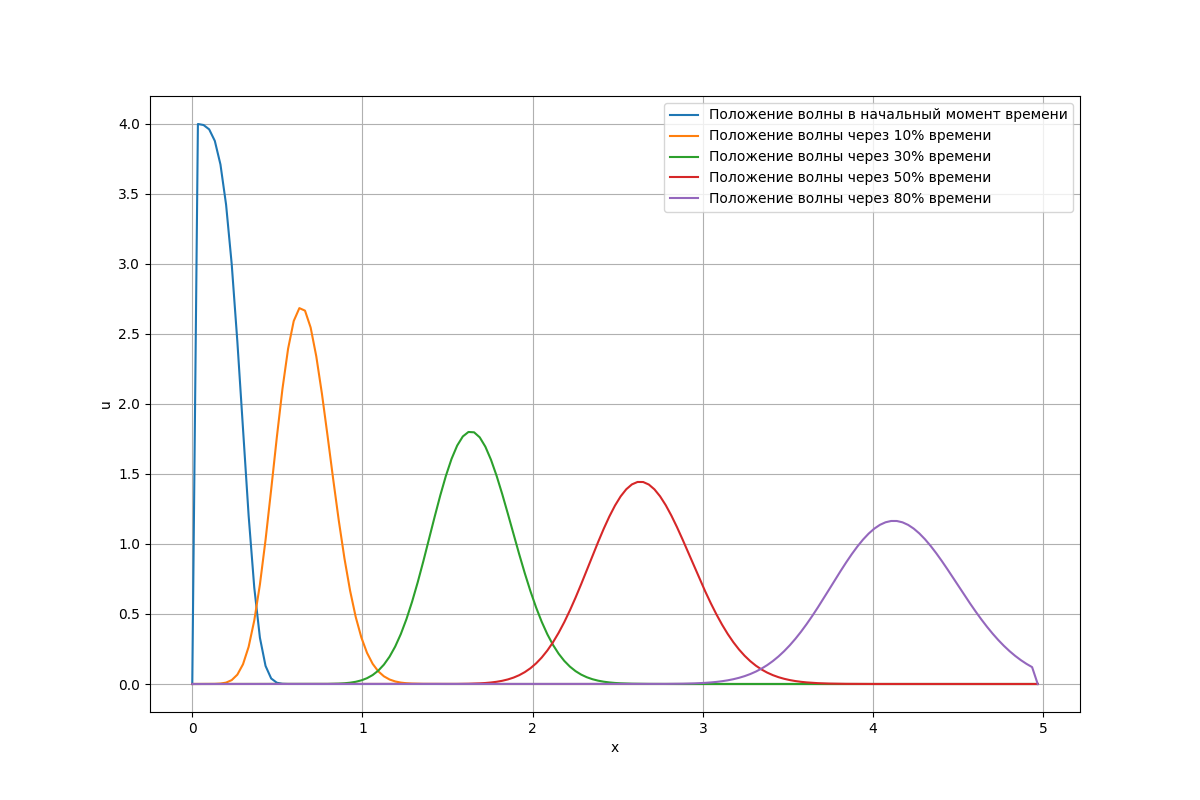
\includegraphics[height=0.7\textwidth]{imgs/upwind_1.5x.png}  % Вставка изображения
	\caption{Результат решения  схемы "вверх по потоку". $\Delta x = 0.05 / 1.5, \Delta t = 0.001$.}  % Подпись к изображению
	\label{fig:upwind_1.5x}  % Метка для ссылки
\end{figure}
Видно (рис \ref{fig:upwind_1.5x}), что пик волны уменьшается медленнее. Форма графика лучше сохраняется
\newpage
Уменьшим шаг по времени в два раза.  Условие CFL выполняется: $\frac{0.001}{0.1} = 0.01 < 1$
\begin{figure}[h]  % Окружение для картинки
	\centering
	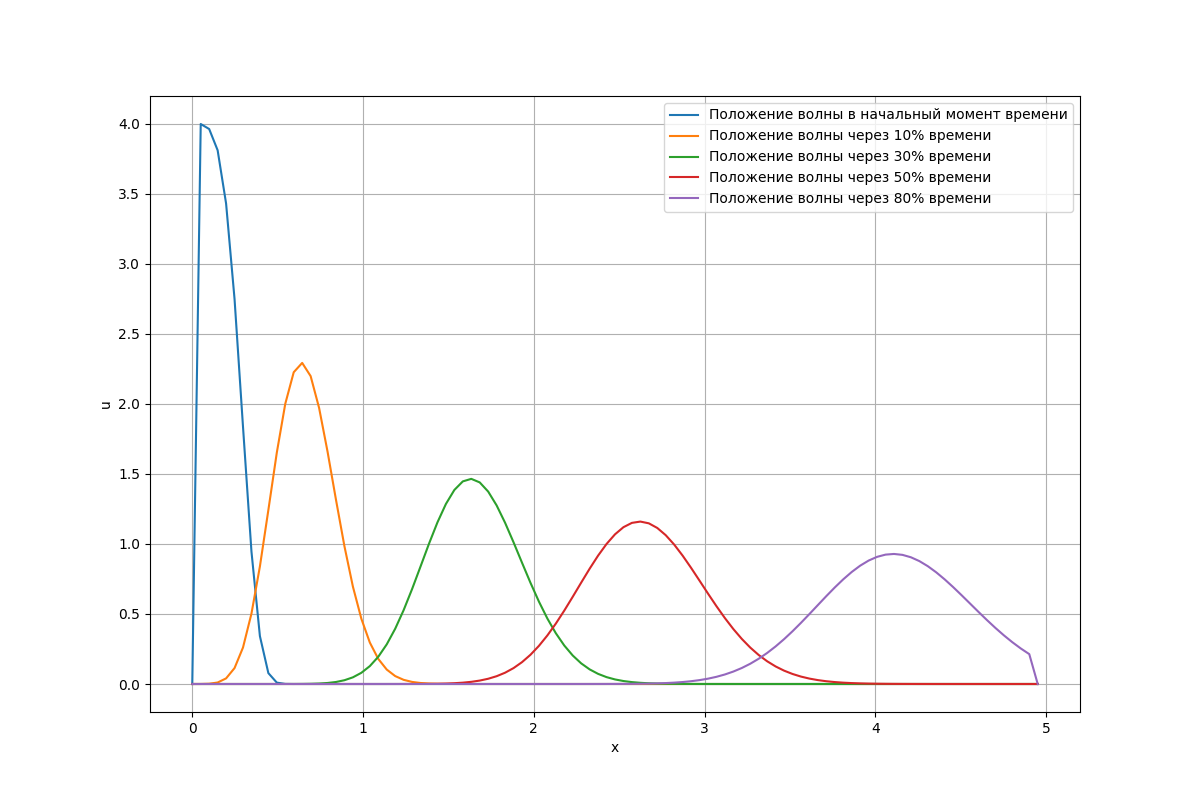
\includegraphics[height=0.7\textwidth]{imgs/upwind_2t.png}  % Вставка изображения
	\caption{Результат схемы "вверх по потоку". $\Delta x = 0.05 , \Delta t = 0.0005$.}  % Подпись к изображению
	\label{fig:upwind_2t}  % Метка для ссылки
\end{figure}

На рис. \ref{fig:upwind_2t} видно, что поведение пика волны не изменилось, отностельно изначальных условий. Форма графика тоже не измненилась








